%% ==========================================================================
%% OpenThomas -- conference version (ACM sigconf, double-blind).
%% BUILD-IN-PUBLIC DRAFT: empirical cells marked \tbd{...} are filled in from
%% the daily pipeline (docs/EXPERIMENTS.md, scripts/paper_data.sh); the
%% conclusions follow the numbers, including the ones against the thesis.
%% Hard limit: <= 8 pages INCLUDING references (over-length = desk reject).
%%
%% CAMERA-READY TODO (revert for the final version):
%%   - remove the `anonymous` and `review` class options;
%%   - restore \settopmatter{printacmref=true} and the copyright permission
%%     block (delete the two suppression lines below);
%%   - fill \acmISBN / \acmDOI / \setcopyright, real author + affiliation;
%%   - restore the repository / project / dataset URLs (footnote below);
%%   - every \tbd{} must be gone, and \draftstatus removed.
%% ==========================================================================
\documentclass[sigconf,review,anonymous]{acmart}

% -- Review-only space savers (RESTORE for camera-ready) --------------------
\settopmatter{printacmref=false}
\renewcommand\footnotetextcopyrightpermission[1]{}
\pagestyle{plain}

% -- Conference metadata (placeholders are fine for review) -----------------
\acmConference[ICAIF '26]{ACM International Conference on AI in Finance}{November 14--17, 2026}{Milan, Italy}
\acmYear{2026}
\copyrightyear{2026}

\usepackage{tikz}
\usetikzlibrary{arrows.meta, positioning, calc, fit, backgrounds}
\definecolor{detfill}{RGB}{224,236,247}
\definecolor{detline}{RGB}{70,120,170}
\definecolor{mdlfill}{RGB}{250,224,190}
\definecolor{mdlline}{RGB}{210,120,30}
\definecolor{srcfill}{RGB}{234,234,234}
\definecolor{srcline}{RGB}{120,120,120}
\definecolor{tbdfill}{RGB}{255,240,200}
\definecolor{tbdline}{RGB}{190,120,0}

% -- Pending-data markers (build-in-public) -----------------------------------
% \tbd{E1}: a number or sentence that the named experiment will supply.
% \pend{text}: a conclusion that stands only if the named experiment agrees.
\newcommand{\tbd}[1]{\colorbox{tbdfill}{\textcolor{tbdline}{\scriptsize\textsf{TBD:#1}}}}
\newcommand{\pend}[2]{\textcolor{tbdline}{#2}\,\tbd{#1}}
% \draftstatus: the build-in-public notice at the top of the body. Remove for camera-ready.
\newcommand{\draftstatus}{\noindent\fcolorbox{tbdline}{tbdfill}{\parbox{\dimexpr\columnwidth-2\fboxsep-2\fboxrule}{%
\footnotesize\textbf{Status of this draft.} This paper is written build-in-public.
The experiments of Section~\ref{sec:results} are pre-registered with their
decision rules; every cell marked \tbd{} is filled from a daily pipeline over a
public, growing dataset, and every sentence marked in \textcolor{tbdline}{orange}
is a conclusion that stands only if the named experiment agrees. Where the data
contradict the thesis, the thesis will be rewritten, not the data.}}\par\medskip}

\begin{document}

\title{The Harness Is the Edge: Leak-Free Evaluation of a Disciplined
Language-Model Agent on Weather Prediction Markets}

\author{Anonymous Author(s)}
\affiliation{%
  \institution{}
  \country{}
}

\begin{abstract}
In the one published benchmark of frontier language models trading real
prediction markets with real capital, all six models lost money. We argue the
failure is a \emph{harness} problem more than a forecasting one: the profitable
signature is selectivity, sized asymmetry, exit discipline, and calibration,
which are properties of the system around the model. We present
\textbf{OpenThomas}, an open-source agent built as that harness and pointed at
the one market category where harness quality is measurable: daily
station-temperature markets on Kalshi and Polymarket, which settle every day
against the U.S.\ National Weather Service climatological report for a named
station. OpenThomas prices each strike from a seven-model numerical-weather
consensus, corrects it by a per-station bias learned from leak-free hindcasts,
widens its uncertainty with its own GenCast ensemble spread, lets a language
model make a \emph{bounded} adjustment, blends with the market prior, and sizes
with fractional Kelly under risk limits the model cannot override. Our main
contribution is methodological: a leak-free replay on real order books with
explicit windows, frozen datasets, local-time decision snapshots, official
NBM/MOS baselines, and day-block bootstrap error bars, together with a
\emph{pre-registered} ablation whose control (the un-blended model with its
edge bar raised to the blend's activity) decides whether the edge is
selectivity or a better probability. A preliminary 21-day replay had found a market-prior
blend positive ($+$\$0.028/contract, 184 trades). The pre-registered replay over
64 settlement days (3{,}349 markets) does not: every setting of the
baseline-only rule loses ($-$\$0.034/contract in production, 95\% CI
$[-0.069, +0.002]$), the blend and a raised edge bar are the same lever
(identical expectancy at matched activity), and the seven-model consensus with
learned station bias is indistinguishable from the NWS National Blend of Models
(Brier 0.163 vs.\ 0.163). What survives is the harness: the drawdown kill-switch
is the one rail that preserved capital under a losing rule, the
self-improvement gate refused most mutations for thin samples and rolled one
promotion back, and station biases persisted out of sample. We report the
result that contradicts our own thesis, and what it changes. All data, frozen
replay rows, and results are published daily.
\end{abstract}

\keywords{prediction markets, large language model agents, autonomous trading,
forecast calibration, numerical weather prediction, backtesting, risk management}

\maketitle

\draftstatus

\section{Introduction}

The obvious way to build a trading agent on top of a large language model (LLM)
is to ask the model what will happen and bet accordingly. The empirical record
so far says this does not work. \emph{Prediction Arena} \cite{predarena} gave
six frontier models \$10{,}000 each and let them trade real prediction markets
autonomously for 57 days. All six lost money, between $-16\%$ and $-30.8\%$.
Research \emph{volume} had no correlation with returns; token spend had none
either. What separated the least-bad runs from the worst was not a better world
model but better \emph{behavior}: being right early, sizing up when confident
and down when uncertain, holding winners to settlement, and, above all, not
trading when there was no edge. The single profitable run on record ($+10.9\%$)
was selective (112 trades), asymmetric (average win \$63.89 vs.\ average loss
\$3.23), and low-drawdown (4.1\%). One benchmark of six models over 57 days is
thin evidence for a universal law; it is, however, exactly the profile a
practitioner would predict, and it motivates the hypothesis this paper sets out
to test rather than assert:

\begin{quote}
\emph{The LLM is not the edge. The harness is the edge.}
\end{quote}

If the edge lives in the harness, progress needs a domain where harness quality
is \emph{measurable}: densely, objectively, and without leakage. Most prediction
markets fail this test: they settle rarely, their resolution is ambiguous, and
any backtest risks letting the replayed market ``know'' something the replayed
model did not. \textbf{Weather markets are the exception.} A daily
station-temperature market (``Will the high in Central Park exceed
83\textdegree{}F today?'') resolves against the NWS climatological report for
one named station, every day, with no interpretive latitude. Dozens of
ground-truth data points arrive per day.

We present \textbf{OpenThomas},\footnote{Open-source; the repository, live
project and dataset URLs are withheld to preserve double-blind anonymity and
will be restored in the camera-ready version.} an open-source ($\approx$8{,}000
lines of Python, 213 tests) agent that operationalizes the harness thesis on
weather markets, and, more importantly, a way of evaluating it that we believe
is the honest one. The paper is written \emph{build-in-public}: the
experiments in Section~\ref{sec:results} are pre-registered with their decision
rules, the numbers are filled from a daily pipeline over a growing public
dataset, and the conclusions follow the numbers. Cells marked \tbd{} are not
yet filled at the time of this draft.

Design commitments:
\begin{itemize}
\item \textbf{Selectivity over activity.} ``No trade'' is the default. The agent
trades only when $|\,\hat{p}-\text{price}\,|$ clears an explicit expected-value
threshold after fees and spread.
\item \textbf{A statistical baseline the model may adjust but never replace.}
Every strike is priced from a seven-model NWP consensus, corrected by
per-(station, lead) bias and spread learned from leak-free hindcasts, and
hard-truncated by what today's thermometer has already locked in. The LLM is
clamped to $\pm 0.15$ around this baseline.
\item \textbf{Hard risk constraints outside the model.} Fractional Kelly sizing,
per-market / per-event / per-category caps, a fee-aware EV threshold, a
longshot-zone filter, and a drawdown kill-switch are deterministic code.
\item \textbf{Calibration as a first-class metric,} tracked per (station, lead)
as Brier skill against the market.
\item \textbf{Self-improvement as a gated loop} with the evaluator structurally
off the agent's edit surface (Section~\ref{sec:rsi}).
\end{itemize}

We contribute: (1) the harness-is-the-edge thesis as a concrete system and a
\emph{pre-registered, falsifiable} test of it (Section~\ref{sec:results}, E1);
(2) a leak-free hindcast/replay methodology for market agents, with explicit
windows, frozen and hashed datasets, local-time snapshots, official-guidance
baselines (NBM, GFS MOS) and day-block bootstrap error bars
(Section~\ref{sec:eval}); and (3) a self-improvement architecture whose safety
comes from a kernel/agent plane split that keeps the judge off the edit
surface, with its empirical record (promotions, rollbacks, vetoes) reported as
it accrues (Section~\ref{sec:rsi}).

\section{Background and related work}

\paragraph{LLMs as forecasters and traders.} A growing literature evaluates
LLMs as probabilistic forecasters. Retrieval-augmented systems approach, but
do not exceed, aggregate human forecasters \cite{halawi2024}; LLM ensembles
match crowd accuracy on some question sets \cite{schoenegger2024}; and the
consistent practical finding is that a \emph{pure} LLM forecast underperforms
the market while a \emph{blend} of model and market price can beat either
\cite{blend}. Prediction Arena \cite{predarena} extends this to live
autonomous trading and finds uniform losses, isolating behavioral rather than
epistemic failure. We take the blend result and the behavioral diagnosis as
design inputs, and we test, rather than assume, which of the two carries the
edge (E1).

\paragraph{Statistical post-processing of weather forecasts.} Learning a
per-station correction to model output is Model Output Statistics
\cite{mos1972}, in operational use for fifty years; the NWS's National Blend
of Models (NBM) \cite{nbm} is a bias-corrected multi-model blend published for
exactly the stations these markets settle on, and GFS MOS bulletins are archived
for every cycle. Our baseline is a small MOS: a shrunken mean error per
(station, kind, lead) on a seven-model consensus. Whether it adds anything over
what the market already reads is an empirical question we answer by pricing the
same markets from NBM and GFS MOS (E5) rather than assuming a ``local edge.''
Machine-learned global models now match or exceed physics-based systems:
GraphCast \cite{graphcast} gives deterministic 10-day forecasts, GenCast
\cite{gencast} calibrated ensembles via diffusion. OpenThomas runs both on
commodity accelerators; GraphCast is a voter in the consensus and GenCast's
ensemble spread is a flow-dependent multiplier on the baseline's $\sigma$.

\paragraph{Sizing, calibration, microstructure.} Fractional Kelly sizing
\cite{kelly} and Platt scaling \cite{platt} are standard; we use them as such.
The favorite--longshot bias \cite{longshot} is encoded as a hard price-zone
filter. Cross-venue listing of the same event (Polymarket vs.\ Kalshi) creates
episodic arbitrage, which the scanner flags deterministically.

\paragraph{Self-improving agents.} A recent framing of near-term recursive
self-improvement (RSI) locates the leverage in the \emph{harness} and names
evaluator strength as the first bottleneck \cite{harness}. The Darwin G\"odel
Machine \cite{dgm} keeps an archive of past variants as mutation parents.
OpenThomas adopts both and adds a security model: because weather markets
supply an unusually strong evaluator, the risk is a \emph{gameable} judge, so
the judge is made structurally unwritable by the optimizer.

\section{Why weather markets are a strong-evaluator domain}
\label{sec:weather}

\textbf{Dense, objective settlement.} Each market resolves against the NWS
Climatological Report (product \texttt{CLI}) for one named station, once per
day: a single integer, the day's observed maximum or minimum. A generalist
agent might see a few dozen settlements per \emph{year}; a weather desk on ten
U.S.\ cities (highs and lows) sees dozens per \emph{day}.

\textbf{A learnable, local correction.} Markets settle on a \emph{specific}
station (NYC $=$ Central Park; Chicago $=$ Midway), and global models have
systematic, station-specific errors there. Throughout, bias is defined as
$b = \text{settled} - \text{consensus}$, so a positive $b$ means the models run
\emph{cold}. Our first 90-day hindcast found Miami $b \approx +1.8$ to
$+2.1$\textdegree{}F ($\sigma\,1.7$), Philadelphia $+2.3$, and LAX $\approx -1$
(models warm). Whether these persist (E9) and whether they beat NBM's own
correction (E5) are measured, not assumed.

\textbf{Leak-free reproducibility.} Historical ``as-of'' forecasts (what a
model published at a past issue time) and historical order books are both
available, so a backtest can present the replayed agent with exactly what it
would have had, and no more. That is what lets us evaluate the \emph{decision
rule}, and later self-improvement, without the replay silently cheating. These
are the properties the RSI literature asks for and rarely gets \cite{harness}.

\section{System architecture}
\label{sec:arch}

OpenThomas is a stack of layers with a strict rule about who is in control at
each one (Figure~\ref{fig:pipeline}, Table~\ref{tab:layers}). Everything that
touches money is deterministic code; the language model is confined to a
bounded adjustment in the middle of the trade path.

\begin{figure*}[t]
\centering
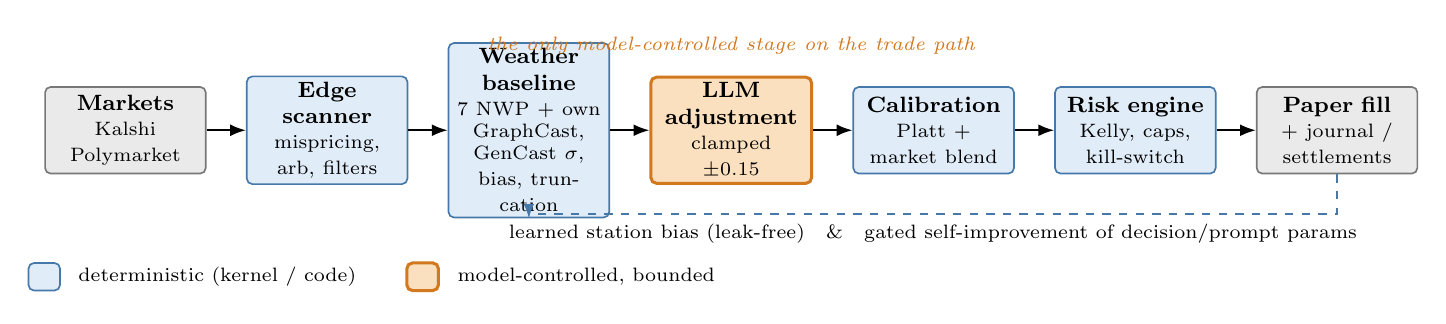
\begin{tikzpicture}[
  font=\footnotesize,
  box/.style={draw, rounded corners=2pt, align=center, minimum height=11mm,
              inner sep=2pt, text width=19mm, line width=0.6pt},
  det/.style={box, fill=detfill, draw=detline},
  mdl/.style={box, fill=mdlfill, draw=mdlline, line width=1.1pt},
  src/.style={box, fill=srcfill, draw=srcline},
  flow/.style={-{Latex[length=2mm]}, line width=0.7pt},
  fb/.style={-{Latex[length=1.8mm]}, dashed, line width=0.7pt, draw=detline},
  node distance=5mm,
]
\node[src] (mk) {\textbf{Markets}\\[1pt]\scriptsize Kalshi\\\scriptsize Polymarket};
\node[det, right=of mk] (scan) {\textbf{Edge}\\\textbf{scanner}\\[1pt]\scriptsize mispricing,\\\scriptsize arb, filters};
\node[det, right=of scan] (base) {\textbf{Weather}\\\textbf{baseline}\\[1pt]\scriptsize 7 NWP + own\\\scriptsize GraphCast, GenCast $\sigma$,\\\scriptsize bias, truncation};
\node[mdl, right=of base] (llm) {\textbf{LLM}\\\textbf{adjustment}\\[1pt]\scriptsize clamped\\\scriptsize $\pm 0.15$};
\node[det, right=of llm] (cal) {\textbf{Calibration}\\[1pt]\scriptsize Platt +\\\scriptsize market blend};
\node[det, right=of cal] (risk) {\textbf{Risk engine}\\[1pt]\scriptsize Kelly, caps,\\\scriptsize kill-switch};
\node[src, right=of risk] (fill) {\textbf{Paper fill}\\[1pt]\scriptsize + journal /\\\scriptsize settlements};

\foreach \a/\b in {mk/scan, scan/base, base/llm, llm/cal, cal/risk, risk/fill}
  \draw[flow] (\a) -- (\b);

\draw[fb] (fill.south) -- ++(0,-5mm) -| node[pos=0.25, below, font=\scriptsize]
  {learned station bias (leak-free) \; \& \; gated self-improvement of decision/prompt params} (base.south);

\node[mdlline, font=\scriptsize\itshape, above=1.5mm of llm] {the only model-controlled stage on the trade path};

\begin{scope}[shift={($(mk.south west)+(0,-13mm)$)}]
  \node[det, minimum height=3.5mm, minimum width=4mm, text width=0pt, inner sep=0pt] (l1) {};
  \node[right=1mm of l1, font=\scriptsize] (l1t) {deterministic (kernel / code)};
  \node[mdl, right=5mm of l1t, minimum height=3.5mm, minimum width=4mm, text width=0pt, inner sep=0pt] (l2) {};
  \node[right=1mm of l2, font=\scriptsize] {model-controlled, bounded};
\end{scope}
\end{tikzpicture}
\caption{The OpenThomas pipeline. A trade flows left to right; the one
model-controlled stage on the trade path is clamped to the statistical baseline
$\pm 0.15$ and bracketed by deterministic layers. (The post-settlement
reflection that distills playbook rules is also model-written, but off the
trade path and human-auditable.) Settled outcomes feed back to teach the
baseline each station's bias (strictly leak-free) and to gate self-improvement
of decision and prompt parameters. Sizing and exposure never leave
deterministic code.}
\label{fig:pipeline}
\end{figure*}

\begin{table*}[t]
\centering
\small
\begin{tabular}{@{}p{2.4cm}p{10.2cm}p{2.9cm}@{}}
\toprule
\textbf{Layer} & \textbf{What it does} & \textbf{Who's in control} \\
\midrule
Edge scanner & Filters markets to plausible mispricings; flags cross-venue arbitrage and longshot / resolution-trap zones & deterministic code \\
Weather baseline & Seven-model NWP consensus $+$ own GraphCast $\to$ per-strike probability at the settlement station, with per-(station, kind, lead) bias/$\sigma$ from leak-free hindcasts, GenCast spread as a $\sigma$ multiplier, and hard truncation by today's observed extreme & deterministic code \\
Forecast engine & LLM ensemble (median of $N$ independent estimates), grounded in resolution rules and base rates, \emph{clamped to baseline $\pm 0.15$} & your choice of model \\
Calibration & Platt-scales forecasts against your own settled history; blends with the market prior & deterministic code \\
Risk engine & Fractional Kelly, per-market/event/category caps, fee-aware EV threshold, longshot filter, drawdown kill-switch & deterministic code \\
Memory & Every forecast and fill journaled to SQLite; post-settlement reflection distills bounded playbook rules & agent, human-auditable \\
\bottomrule
\end{tabular}
\caption{The OpenThomas stack. The model \emph{proposes}; the risk engine
\emph{disposes}. One layer on the trade path is model-controlled, bounded
above and below by deterministic layers.}
\label{tab:layers}
\end{table*}

\paragraph{Market connectors and paper simulation.}
A unified \texttt{Market}/\texttt{Order}/\texttt{Position} model spans Polymarket
(Gamma API for discovery, CLOB for books/orders) and Kalshi (REST $+$ WebSocket,
RSA-signed, CFTC-regulated). A \emph{paper} connector wraps either venue's real
market data but simulates fills locally at bid/ask (never mid), with
mark-to-market at bid (liquidation value). Paper mode is the default and needs
no exchange keys.

\paragraph{The weather baseline.}
For a market on station $s$, valid day $d$, kind $k\in\{\text{high},\text{low}\}$,
the baseline forms a consensus temperature $\bar{T}$ across seven operational
global models (GFS, ECMWF-IFS, ICON, GEM, UKMO, M\'et\'eo-France, JMA) plus the
system's own GraphCast point forecast, with cross-model spread
$\sigma_{\text{model}}$, and applies two corrections learned strictly
out-of-window:
\[
\hat{T} = \bar{T} + b_{s,k,\ell}, \qquad
\sigma = \max\!\big(\sigma_{s,k,\ell},\, 0.8\,\sigma_{\text{model}}\big)\cdot g_{s,d},
\]
where $\ell$ is the forecast lead, $b_{s,k,\ell}$ the learned bias,
$\sigma_{s,k,\ell}$ the residual spread (both shrunk toward a climatological
prior with pseudo-count 10), and $g_{s,d}\in[0.7,1.6]$ the GenCast
flow-dependent multiplier (the day's ensemble spread relative to a typical day
at that lead; GenCast's 12-hour steps undersample the diurnal peak, so it
contributes uncertainty, not a point estimate). The per-strike probability is
the mass on the correct side of the half-integer strike under a fat-tailed
mixture ($0.8\,\mathcal{N}(\hat T,\sigma) + 0.2\,\mathcal{N}(\hat T,2\sigma)$),
with one more hard step: \emph{truncation}. If today's thermometer has already
made one side impossible, the probability is clamped accordingly. This is where
a naive backtest leaks, and where Section~\ref{sec:eval} spends most of its
care.

\paragraph{Forecast engine: bounded LLM adjustment.}
The model receives the baseline probability, resolution rules, base rates, and a
news brief, and returns an adjusted probability, then \emph{clamped to baseline
$\pm 0.15$}. The statistics do the heavy lifting; the model is there for what the
statistics cannot see (a blown front, a stale consensus, a discontinuity in the
question text). Because of the clamp, mid-size local reasoning models suffice,
which keeps the agent runnable on self-hosted open-weights models. Whether the
adjustment adds anything, and at which clamp, is E4.

\paragraph{Calibration and market-prior blend.}
Once $\geq 30$ markets settle in a category, OpenThomas fits Platt scaling, then
blends the calibrated forecast with the market price:
$p = w\cdot\text{mid} + (1-w)\cdot\hat p$, $w = 0.5$ in production. The blend
weight and the minimum edge are entry-\emph{selectivity} parameters and are
candidates for self-improvement under kernel bounds (Section~\ref{sec:rsi});
sizing is not.

\paragraph{Risk engine (deterministic).}
The engine takes bankroll, risk profile, the blended probability, and market
price/liquidity, and returns an approved size or a rejection naming the binding
constraint: fractional Kelly ($0.15\times$ to $0.33\times$ by profile),
per-market (5\%), per-event (10\%) and per-category (25\%) caps at cost basis,
50\% total open risk, a fee-aware EV threshold, a $[0.05, 0.95]$ price zone, a
solvency check, and a drawdown kill-switch (15\%) that halts trading until a
human resumes. None of these are reachable by the model or by the
self-improvement loop; a kernel policy test fails any change that tries to
move a safety rail into the optimizer's reach. What each rail costs or saves
on the replayed trades is E7.

\section{Self-improvement with the judge off the edit surface}
\label{sec:rsi}

OpenThomas updates OpenThomas. The operator is moved \emph{up} the stack, setting
bounds and reviewing lineage, and is forbidden from hand-tuning trading
parameters. The design problem is that self-improvement is safe only if
improvement cannot redefine ``improvement'': an optimizer that can edit its own
judge will find it easier to lower the bar than to clear it.

\paragraph{Kernel/agent planes.} The codebase is split into two planes, and the
split \emph{is} the security model (Table~\ref{tab:planes}). The \textbf{kernel}
plane (promotion gate, parameter bounds, the risk engine and all safety rails,
the truth pipeline, the journal schema) is written only by the operator; the
evolution loop has no write path to it. The \textbf{agent} plane
(decision-rule parameters, the forecast prompt template; on the roadmap,
workflow structure and strategy code) is written by the evolution loop, only
\emph{through} the kernel gate. Entry-selectivity knobs (minimum edge, blend
weight) are genome parameters under kernel bounds; sizing, exposure caps and
the kill-switch can never enter the parameter space.

\begin{table}[t]
\centering
\small
\begin{tabular}{@{}p{1.3cm}p{4.2cm}p{1.7cm}@{}}
\toprule
\textbf{Plane} & \textbf{Contents} & \textbf{Written by} \\
\midrule
kernel & bounds, promotion gate, risk engine \& safety rails, truth pipeline, journal schema & operator only \\
agent & decision-rule params, forecast prompt template; later: workflow, strategy code, the evolver & evolution loop, \emph{via the gate} \\
\bottomrule
\end{tabular}
\caption{The plane split is the security model: the judge is not on the
optimizer's edit surface.}
\label{tab:planes}
\end{table}

\paragraph{Loops and the gate.} A fast \emph{trading} loop (minutes) runs the
champion parameters. A \emph{reflection} loop (on settlements) distills bounded
playbook rules. An \emph{evolution} loop mines failure evidence from the
journal, proposes mutations (LLM-directed, plus Gaussian mutations from an
archive of past variants \cite{dgm}) and submits them to the gate, which scores
a candidate \emph{strategy callable} on leak-free replay with four anti-gaming
properties: \emph{held-in/held-out} splits (winners are picked on older days;
the freshest seven days only veto, and the window rolls forward daily);
\emph{totals-not-ratios} with a minimum trade count (a rule that trades twice
cannot win on ratio; one that trades nothing cannot win on drawdown);
\emph{out-of-sample regret rollback} (each cycle re-scores the active generation
against its parent on the fresh window and reverts if the parent now wins); and
a \emph{Brier veto} for the forecast operator (a prompt that wins PnL while
worsening calibration got lucky). Each of the four is a unit test in the
repository. Generation 0 is the operator's config: the human's settings win
until the loop has promoted evidence-backed changes past them.

\paragraph{Empirical status.} The architecture is shipped; its record is
short. Over 18 daily meta-cycles (2026-07-10 to 09-06) the loop recorded 3
promotions, 1 rollback and 0 Brier vetoes (Table~\ref{tab:lineage}); of the
candidates it scored, most (25 of 38) were refused for the thin-sample rule
(held-in $n<20$), which is the gate doing its job on a small window rather than
the loop learning. The one promotion that reached the fresh window with a
worse record than its parent was reverted two days later. We make no claim
that the loop has improved trading: the active generation
(min\_edge $0.15$, $w=0.6$) scored $-$\$3.00 held-in against the champion's
$-$\$6.22, i.e.\ it lost less. Improvement axes are unified as
mutation operators feeding the same accept mechanism: playbook rules and
calibration refits, decision-parameter and prompt mutation (shipped), then
workflow structure, then agent-plane code diffs (adding shadow trading and
human diff review), then LoRA adapters with a time-discounted reward. The
admission rule is strict: a parameter enters the space only when the gate can
discriminate on it. \emph{Tuning what you cannot measure is drift, not
improvement.}

\section{Leak-free evaluation methodology}
\label{sec:eval}

The hardest part of evaluating a market agent is not computing PnL; it is not
lying to yourself. \texttt{hindcast} teaches the baseline each station's bias
from archived as-of forecasts (the previous-runs API of a public NWP aggregator)
and official settlements, strictly \emph{before} any window it is evaluated on.
\texttt{replay} then backtests the \emph{decision rule} against real historical
order books, drawing prices from hourly candlesticks at a decision snapshot,
and freezes every decision-time row (baseline probability, bid/ask at the
snapshot, outcome) to a hashed file that every later experiment re-scores.

\paragraph{Snapshots are local, and the replay is asymmetric on purpose.} The
NWS CLI day is a \emph{local} calendar day, so the snapshot is a local hour: for
lows, local midnight, the first minute of the day, when nothing of the minimum
can be on the books (a fixed 06Z, which we used first, was 2am on the east
coast, two hours into the day); for highs, 11:00 local, when the afternoon peak
is still a live contest. The governing rule, learned when an early backtest
snapshotted the dawn low after it had been realized, is \emph{never let the
replayed market know something the replayed model does not}. The converse is
allowed and is the case here: by 11:00 the book has already digested the
morning's observations, while the replayed model is stripped of intraday
observations, same-day model runs, the LLM adjustment and the calibration layer.
The replay therefore \emph{handicaps} the model. Its numbers are a conservative
bound on the decision rule, not a fair contest between the model and the crowd,
and the ``naked model'' row of E1 must be read that way. Sensitivity to the
snapshot hour is E3.

\paragraph{Official baselines.} A learned station correction is a small MOS.
The obvious question, ``is it better than what the market already reads?'', is
answered by pricing the same markets, with the same decision rule and the same
out-of-window bias learning, from NBM and from GFS MOS bulletins archived as
issued (the $d\!-\!1$ 12Z cycle, about a day ahead, matching the consensus'
lead-1 guidance) (E5).

\paragraph{Error bars.} Markets on one day share a thermometer and a synoptic
pattern, so trades are not independent. Every PnL-per-contract figure carries a
95\% interval from a block bootstrap that resamples settlement \emph{days}, a
$t$-statistic on daily PnL, and the maximum drawdown of the daily path.

\paragraph{The gate uses the same pipeline.} The row collector that scores a
candidate generation is the one that enforces no-peeking, and it lives in the
kernel where the optimizer cannot touch it.

\section{Pre-registered experiments and results}
\label{sec:results}

\paragraph{Protocol.} Window: settlement days from 2026-07-09 (the first day
with archived lead-1 guidance for every station) to \tbd{E1}, rolling
forward daily; ten U.S.\ stations, twelve Kalshi daily-temperature series
(nine highs, three lows); station bias/$\sigma$ learned only from days before
the window start; fees included (Kalshi taker: $\lceil 7\%\cdot p(1-p)\rceil$
cents per contract); production parameters min\_edge $=0.08$, $w=0.5$, lead 1.
Every table names the frozen dataset (file, SHA-256 prefix) it was scored on.
Table~\ref{tab:prereg} lists the experiments and, crucially, what each one
\emph{decides}; the decisions were written before the numbers.

\begin{table*}[t]
\centering
\small
\begin{tabular}{@{}p{0.5cm}p{7.6cm}p{8.4cm}@{}}
\toprule
\# & \textbf{Experiment} & \textbf{Decision rule (written before the data)} \\
\midrule
E1 & Ablation: naked model $\to$ $+$station bias $\to$ $+$market blend $\to$ \textbf{control}: no blend, edge bar raised until it trades as rarely as the blend & If the control's PnL/ct is positive with a 95\% CI excluding zero, \emph{selectivity} is the edge. If only the blended row is, the edge is the \emph{blend} (a better probability) and the thesis sentence changes to say so. \\
E2 & Grid: min\_edge $\times$ blend weight & The E1 conclusion must hold across neighbouring cells, not one. \\
E3 & Snapshot sensitivity: lows at local 00/01/02, highs at 09/11 & If PnL/ct moves by more than its CI half-width, timing is doing work and the leak-free claim is weakened accordingly. \\
E4 & LLM on/off; clamp $\delta\in\{0,.05,.10,.15,.25,\infty\}$; PnL and Brier & Whether the bounded adjustment adds anything over the baseline, and at which $\delta$; Brier must not worsen. \\
E5 & Same decision rule priced from NBM and GFS MOS, each with its own learned bias & If NBM ties the consensus, ``learnable local edge'' is dropped from the paper. \\
E6 & Breakdown by station, ISO week, high/low & Whether the edge is broad or one station in one week. \\
E7 & Sizing regimes on the production trades: flat, Kelly, Kelly$+$caps, Kelly$+$caps$+$kill-switch & What each rail costs or saves: the only numbers the ``harness'' layer gets. \\
E8 & Self-improvement lineage over $\geq 4$ weeks: promotions, rollbacks, vetoes & Whether Section~\ref{sec:rsi} keeps an empirical claim or becomes future work. \\
E9 & Station bias on first vs second half of the hindcast window & Whether ``biases persist'' is true (same sign, similar magnitude). \\
\bottomrule
\end{tabular}
\caption{Pre-registered experiments. Each is one command over the frozen
dataset; results are regenerated daily and published with the data.}
\label{tab:prereg}
\end{table*}

\paragraph{Preliminary replay (v0, superseded).} Before the protocol above was
fixed, a 21-day replay (968 settled markets, 2026-06-24 to 07-14, UTC
snapshots 06Z/15Z, no error bars) gave: naked model-vs-market
$-$\$0.007/contract over 425 trades (41\% wins); $+$learned bias
$-$\$0.005 over 396; $+$market-prior blend $+$\$0.028 over 184 (45\% wins).
The blend more than halved activity and flipped expectancy positive. That is
consistent with the thesis, but it is also consistent with the blend simply
being a better probability, and 184 trades in one three-week window carries no
error bar. It motivated E1's control and is not used for any conclusion below.

\paragraph{E1: ablation with the selectivity control.}
Table~\ref{tab:ablation}. Every row loses. The learned station bias helps a
little ($-0.041 \to -0.037$); the blend helps a little more ($-0.034$) and
halves activity; and the control, the un-blended model with its edge bar raised
from $0.08$ to $0.19$ until it trades as rarely as the blend, lands on the
\emph{same} expectancy ($-0.034$, $n=618$ vs.\ $625$) with an interval that
includes zero on both. The pre-registered rule therefore returns neither
answer: the blend and selectivity are one lever, and neither produces positive
expectancy with this baseline. The v0 result ($+$\$0.028 over three weeks) does
not reappear: the same weeks in this dataset are $+0.004$ (W28) and $+0.074$
(W30) against $-0.066$ (W29), and the 64-day mean is negative.

\begin{table}[t]
\centering
\small
\begin{tabular}{@{}p{3.1cm}rrrr@{}}
\toprule
\textbf{Rule} & \textbf{n} & \textbf{PnL/ct} & \textbf{95\% CI} & \textbf{maxDD} \\
\midrule
Naked model vs market & 1501 & $-0.041$ & $[-0.058, -0.023]$ & 61.8 \\
\quad $+$ learned station bias & 1407 & $-0.037$ & $[-0.056, -0.016]$ & 55.5 \\
\quad\quad $+$ market blend (prod.) & 625 & $-0.034$ & $[-0.069, +0.002]$ & 23.7 \\
Control: no blend, bar $0.19$ & 618 & $-0.034$ & $[-0.070, +0.002]$ & 23.2 \\
\bottomrule
\end{tabular}
\caption{E1 on the frozen dataset (window 2026-07-09 to 09-10, digest
7c3fb9f21ab727e3), 64 settlement days, 3{,}349 rows, win rates 37--38\%
throughout. CI: day-block bootstrap. maxDD: of the daily PnL path, \$
per one contract per trade.}
\label{tab:ablation}
\end{table}

\paragraph{E2--E3: robustness.} Of the 31 grid cells with at least 18 trades,
all 31 are negative (range $-0.029$ to $-0.140$/contract); the only positive
cell ($w=0.75$, min\_edge $0.15$) has six trades. The E1 conclusion is not a
property of one cell. Snapshot sensitivity: \tbd{E3} \emph{(PnL/ct with lows at
local 01:00 and 02:00 and highs at 09:00, vs.\ the E1 half-width)}.

\paragraph{E4: does the LLM add anything?} \tbd{E4} \emph{(table of $\delta$
vs.\ n, PnL/ct, Brier; baseline Brier $0.163$)}. The live paper run gives a
first, unflattering answer (Section~\ref{sec:live}): the live forecaster's
Brier over 41 settled trades is $0.43$ against a market Brier of $0.10$--$0.19$
at the same stations, so the adjustment the live agent actually made hurt
calibration. \pend{E4}{Whether a clamped adjustment on the replay rows does the
same is what the sweep decides.}

\paragraph{E5: against the official guidance.} On the same 3{,}349 markets,
priced by the same rule with each source's own out-of-window bias: the
seven-model consensus scores Brier $0.1627$, NBM $0.1631$, GFS MOS $0.1651$
($n=3{,}344$ paired); PnL/contract $-0.034$, $-0.055$ $[-0.088, -0.021]$, and
$-0.035$ $[-0.069, +0.001]$. The consensus with learned bias ties NBM.
\textbf{We drop the ``learnable local edge'' claim:} the correction is real
(E9) but it recovers what the NWS's own blend already publishes, and the
market reads that.

\paragraph{E6: where the edge lives.} Four of ten stations are positive
(Chicago $+0.071$, $n=59$; Miami $+0.040$; New York $+0.033$; San Antonio
$+0.015$, $n=29$) and six negative (Atlanta $-0.147$, Denver $-0.093$, Austin
$-0.065$, Los Angeles $-0.064$, Philadelphia $-0.049$, Dallas $-0.022$); three
of ten weeks are positive. Lows ($-0.006$, $n=71$) lose less than highs
($-0.038$, $n=554$), consistent with the local-midnight snapshot leaving the
low a genuinely open contest while the 11:00 book already knows the morning.
None of the positive stations' intervals exclude zero on their own.

\paragraph{E7: the harness, scored.} The 625 production trades through the
risk engine on a \$1{,}000 paper bankroll (Table~\ref{tab:sim}). With a losing
rule, sizing is a multiplier on the loss: flat 1\% stakes lose 10\%, fractional
Kelly 23\% with a 71\% drawdown, and the concentration caps change which losses
are taken rather than whether ($-42\%$: they cut the winners' size on
multi-strike days as much as the losers'). The kill-switch is the rail that
mattered: it halted trading on 2026-07-17 after 11 entries, refused the next
547, and ended the window at $+12\%$ with a 15\% drawdown, which is the
honest reading of ``the harness is the edge'' on this data: the harness did not
create an edge, it stopped a losing rule from compounding.

\begin{table}[t]
\centering
\small
\begin{tabular}{@{}lrrrl@{}}
\toprule
\textbf{Sizing} & \textbf{Return} & \textbf{maxDD} & \textbf{Entered} & \textbf{Halted} \\
\midrule
Flat 1\% & $-10.2\%$ & 22.8\% & 88 & --- \\
Kelly $0.15\times$ & $-23.3\%$ & 70.5\% & 88 & --- \\
Kelly $+$ caps & $-41.5\%$ & 77.2\% & 88 & --- \\
Kelly $+$ caps $+$ kill-switch & $+12.0\%$ & 15.2\% & 11 & 07-17 \\
\bottomrule
\end{tabular}
\caption{E7: the same 625 trades under each sizing regime (conservative
profile: Kelly $0.15\times$, caps 5/10/25/50\%, kill-switch at 15\% drawdown;
537 of the trades fail the live engine's fee-aware edge check at their
snapshot price and are never entered). ``Entered'' counts positions opened.}
\label{tab:sim}
\end{table}

\paragraph{E8--E9.} The lineage is Table~\ref{tab:lineage}. Station bias
persists: on lead-1 highs and lows, 11 of 12 (station, kind) biases keep their
sign between the first 123 verified days and the last 32 (the exception,
Chicago Midway, is $-0.1$ vs.\ $+0.3$, i.e.\ zero both times), and magnitudes
hold (Miami $+2.0 \to +1.8$, Philadelphia $+2.6 \to +1.6$, Atlanta
$+2.4 \to +2.1$, LAX $-1.0 \to -1.2$, Austin low $-2.1 \to -3.8$). The
correction is real; E5 says the market already has it.

\begin{table}[t]
\centering
\small
\begin{tabular}{@{}rrlllrrl@{}}
\toprule
\textbf{gen} & \textbf{par.} & \textbf{by} & \textbf{edge} & \textbf{$w$} & \textbf{in} & \textbf{out} & \textbf{status} \\
\midrule
0 & --- & oper. & $0.08$ & $0.5$ & --- & --- & baseline \\
1 & 0 & LLM & $0.12$ & $0.6$ & $+2.31$ & $+1.63$ & prom.\ 07-23 \\
2 & 1 & rand. & $0.115$ & $0.59$ & $+9.22$ & $+1.16$ & 07-25, reverted \\
3 & 1 & LLM & $0.15$ & $0.6$ & $-3.00$ & $-1.32$ & 09-01, active \\
\bottomrule
\end{tabular}
\caption{E8: self-improvement lineage as exported by the loop (18 meta-cycles,
2026-07-10 to 09-06). edge: min\_edge; $w$: market-prior weight; in/out:
held-in and held-out total PnL (\$) at promotion. Generation 2 was reverted when its
parent beat it on the rolled-forward window.}
\label{tab:lineage}
\end{table}

\paragraph{The live paper run.}
\label{sec:live}
The reference agent has paper-traded continuously since July (1{,}911 cycles,
\$100{,}000 allocated) with every live-only advantage on: intraday
observations, same-day model runs, the LLM adjustment, calibration. At the
time of writing: 41 settled trades, realized $-$\$1{,}679, unrealized
$+$\$593, total $-1.1\%$, maximum drawdown $3.0\%$, win rate 24\% with average
win \$243 against average loss \$132. The asymmetry is the harness's; the
expectancy is not there. Its forecaster's Brier ($0.43$) against the market's
($0.10$--$0.19$) is the sharpest single number in this paper.

\section{Discussion and limitations}

\paragraph{The claims are only as wide as the window.} The replay is paper
mode at real bid/ask; it is an ablation over one summer season, not a track
record. The live paper run is the ongoing public test, reported with wins and
losses alike, and this paper's tables are regenerated from it daily.

\paragraph{What the replay cannot see.} Replay has no news brief, no intraday
observations, no forecaster-discussion text, and (except in E4) no LLM and no
calibration layer; it measures the decision rule over the statistical baseline,
the dominant live pathway for weather markets, but not the whole live agent. A
residual leak risk, an LLM ``remembering'' recent weather from pre-training, is
negligible with a local model whose cutoff precedes the window, and must be
rechecked whenever the forecaster is swapped.

\paragraph{Capacity is the real ceiling.} Daily-temperature markets are thin. A
survey of seven Kalshi cities found on the order of a few hundred thousand
dollars of daily notional in aggregate, which bounds extraction at low
single-digit millions per year even under optimistic assumptions. This is a
methodology contribution about \emph{measurable} edge, not a claim of scalable
returns.

\paragraph{Generalization.} The strong-evaluator property is what makes weather
the right first domain; it is also what most other markets lack. Extending the
harness and the gate to weaker-evaluator markets is future work; the journal
already archives each live forecast's inputs so a trace-replay evaluator can
begin to close that gap.

\section{Reproducibility, ethics, and broader impact}

The system, the evaluation pipeline, the frozen replay datasets with their
digests, the experiment results, and the as-of forecast record (NWP guidance,
settlements, own GraphCast/GenCast rows, NBM/MOS baselines) are public and
updated daily; paper mode requires no exchange keys and reproduces every table
from the published files (Appendix~\ref{app:repro}). Live trading is off by
default and requires two independent explicit opt-ins; the agent has no
deposit, withdrawal, or transfer capability. We ship hard position limits and a
drawdown kill-switch, and we state plainly that no software makes trading safe:
roughly 70\% of Polymarket addresses have lost money, and every layer of this
paper is about losing less. On the self-improvement side, the safety argument
is architectural rather than behavioral: the judge is off the optimizer's edit
surface by construction, safety rails are outside the parameter space by a
kernel policy test, and every promotion is an auditable commit authored by the
loop itself.

\section{Conclusion}

Autonomous LLM traders have so far lost money, and the profile of the runs that
lost least points at discipline rather than forecasting. OpenThomas puts the
discipline in deterministic code, uses a language model only for a bounded
adjustment, and points the whole system at weather markets, the one category
where the resulting edge can be measured densely, objectively, and without
leakage. The contribution we are surest of is the measurement: explicit
windows, frozen and hashed datasets, local-time snapshots, official baselines,
day-block error bars, and a pre-registered control that can falsify our own
thesis. On 64 days of data the pre-registered test came back against us: no
setting of the baseline-only rule has positive expectancy, the blend and the
edge bar are the same lever, and the learned station correction is what the
NWS blend already publishes. What the harness demonstrably did was limit the
damage: the kill-switch preserved capital, the gate refused thin evidence and
reverted an overfit promotion. A positive edge in this market, if it exists,
needs what the replay strips out and the live agent has not yet turned into
calibration: intraday observations, same-day runs, and a language-model
adjustment that improves Brier rather than worsening it (E4). We report the
result in public, losses included, and invite the community to check it.

\begin{thebibliography}{14}
\bibitem{predarena} J.~Zhang, G.~Liu, O.~Johansson, H.~Yitayew, K.~Ohly, and
G.~Li. Prediction Arena: Benchmarking AI models on real-world prediction
markets. arXiv:2604.07355, 2026.
\bibitem{blend} R.~Alur, B.~C. Stadie, D.~Kang, et al. AIA Forecaster:
Technical report. arXiv:2511.07678, 2025.
\bibitem{halawi2024} D.~Halawi, F.~Zhang, C.~Yueh-Han, and J.~Steinhardt.
Approaching human-level forecasting with language models. arXiv:2402.18563, 2024.
\bibitem{schoenegger2024} P.~Schoenegger, I.~Tuminauskaite, P.~S. Park, and
P.~E. Tetlock. Wisdom of the silicon crowd: LLM ensemble prediction
capabilities rival human crowd accuracy. \emph{Science Advances}, 10(45), 2024.
\bibitem{mos1972} H.~R. Glahn and D.~A. Lowry. The use of Model Output
Statistics (MOS) in objective weather forecasting. \emph{J.\ Applied
Meteorology}, 11(8):1203--1211, 1972.
\bibitem{nbm} T.~M. Hamill, E.~Engle, D.~Myrick, M.~Peroutka, C.~Finan, and
M.~Scheuerer. The U.S.\ National Blend of Models for statistical
postprocessing of probability of precipitation and deterministic
precipitation amount. \emph{Monthly Weather Review}, 145(9):3441--3463, 2017.
\bibitem{graphcast} R.~Lam et al. GraphCast: Learning skillful medium-range global
weather forecasting. \emph{Science}, 382(6677):1416--1421, 2023.
\bibitem{gencast} I.~Price et al. Probabilistic weather forecasting with machine
learning. \emph{Nature}, 637:84--90, 2025.
\bibitem{kelly} J.~L. Kelly. A new interpretation of information rate.
\emph{Bell System Technical Journal}, 35(4):917--926, 1956.
\bibitem{platt} J.~Platt. Probabilistic outputs for support vector machines and
comparisons to regularized likelihood methods. In \emph{Advances in Large
Margin Classifiers}, MIT Press, 1999.
\bibitem{longshot} J.~Whelan et al. The favorite--longshot bias in prediction
markets. SSRN 5502658, 2026.
\bibitem{harness} L.~Weng. Harness engineering for self-improvement. Blog post,
lilianweng.github.io, 2026.
\bibitem{dgm} J.~Zhang, S.~Hu, C.~Lu, R.~Lange, and J.~Clune. Darwin G\"odel
Machine: Open-ended evolution of self-improving agents. arXiv:2505.22954, 2025.
\end{thebibliography}

\appendix
\section{Reproducibility details}
\label{app:repro}

\begin{center}
\small
\begin{tabular}{@{}p{3.2cm}p{4.6cm}@{}}
\toprule
\textbf{Item} & \textbf{Value} \\
\midrule
Stations & KNYC, KAUS, KMDW, KMIA, KLAX, KPHL, KDEN, KDFW, KATL, KSAT \\
Series & 9 daily-high, 3 daily-low Kalshi series \\
NWP guidance & Open-Meteo previous-runs API, hourly 2\,m temperature, models gfs, ecmwf\_ifs025, icon, gem, ukmo, meteofrance, jma; daily extremes over the local day; leads 1--5 \\
Settlements & ACIS daily max/min for the NWS station (the CLI integer) \\
Official baselines & IEM MOS archive, models NBS (\texttt{txn}) and GFS MOS (\texttt{n\_x}), $d\!-\!1$ 12Z cycle \\
Bias/$\sigma$ & shrinkage pseudo-count 10 toward $\sigma_{\text{prior}}(\ell)=\{2.3, 2.8, 3.4, 4.0, 4.6\}$\textdegree{}F for $\ell=1..5$; learned only from days $<$ window start \\
Strike probability & $0.8\,\mathcal N(\hat T,\sigma)+0.2\,\mathcal N(\hat T,2\sigma)$ at half-integer thresholds \\
Snapshot & lows: local 00:00; highs: local 11:00; hourly candle close bid/ask; spread $\le 0.10$ required \\
Decision rule & $p = w\,\text{mid} + (1-w)\hat p$, $w=0.5$; trade the side with $p - \text{price} - \text{fee} \ge 0.08$, price in $[0.05,0.95]$, at most one side per market \\
Fees & Kalshi taker $\lceil 7\,p(1-p)\rceil$ cents per contract \\
Error bars & day-block bootstrap, 2{,}000 resamples, seed 0 \\
Risk profile (E7) & conservative: Kelly $0.15\times$, caps 5/10/25/50\%, kill-switch 15\%; \$1{,}000 bankroll \\
LLM (E4) & \tbd{E4} model id, checkpoint date; temperature 0, single sample, prompt cached by exact text \\
Commands & \texttt{hindcast --days 92}; \texttt{replay --start --end --rows-out}; \texttt{ablate --rows-in --out} \\
\bottomrule
\end{tabular}
\captionof{table}{Everything needed to regenerate the tables from the published files.}
\end{center}

\end{document}
